\section{Network Characteristics of OS Services}
\label{sec:characterize-os}

Mobile operating systems provide APIs and OS level services to optimize network usage.
For example, the Apple Push Notification service (APNs) and Google Cloud Messaging (GCM) are used by iOS applications and Android applications respectively to receive notifications from the Internet.
\tbd{About location services}
In this section we perform a set of controlled experiments to detail the network characteristics of these OS services.
The questions that we answer in this section are as follows.
\begin{packedenumerate}
\item What are the network characteristics of operating system services?
\item How different is the network traffic from iOS devices compared to Android devices?
\item What is the impact of operating system services in the wild? \tbd{rephrase this}
\end{packedenumerate}

\subsection{Traffic from Factory Reset Devices}

We now detail the network characteristics of mobile devices and the pre-installed applications.
We use the following questions to guide our analysis.
\begin{packedenumerate}
\item What is the network usage of devices that are used \emph{out of the box}? 
\item How does the device, manufacturer, and operating system affect the network usage?
\end{packedenumerate}

We answer these questions with a controlled experiment performed on an iPod Touch, an iPad, a Samsung Galaxy SIII, and a Google Nexus S Phone.
Each of these devices were reset to factory default settings after their batteries were fully charged. 
We then allowed these devices to connect to the Internet using our \wifi hotspot.
We ran tcpdump on our hotspot to monitors the Internet traffic from these devices for 3 sessions of 24 hours. 
We add a dummy email account as the primary account on each of these devices. 
This account is responsible for triggering any OS specific services that may require the device to be in use. 
We use the data collected as a rough estimate on the minimum data traffic that is generated by the devices. 
We observed that during the initialization the devices exchanged from 20 MB to 50 MB. 
We now present the traffic characteristic observed during the time after this initialization. 

\begin{table}
\begin{small}
\begin{tabular}{|c|c|c|c|c|}
\hline
\multirow{2}{*}{\bf Application} & \multicolumn{4}{c|}{\bf Traffic Share in the first 24 hours}\tabularnewline
\cline{2-5}
     & iPad & iPod & Galaxy SIII & Nexus \tabularnewline
     & (19 KB) & (21 KB) & (47 KB)& (97 KB)  \tabularnewline
\hline
Notifications & 0.54 & 0.53 & 0.35 & 0.88 \tabularnewline
\hline
Location & 0 & 0 & 0.26 & 0 \tabularnewline
\hline
SSL & 0 & 0 & 0.30 & 0.11 \tabularnewline
\hline
Mail & 0.05 & 0.07 & 0 & 0 \tabularnewline
\hline
HTTP & 0.13 & 0 & 0.09  & 0 \tabularnewline
\hline
UDP & 0.28 & 0.40 & 0.01 & 0.01 \tabularnewline
\hline
{\em total}& {\em 1.0} & {\em 1.0} & {\em 1.0} & {\em 1.0}\tabularnewline
\hline
\end{tabular}
\end{small}
\caption{Network usage in the first 24 hours after factory reset. \emph{Notifications contribute to the largest fraction of traffic volume across all devices.}}
\label{tab:traffic-share-factory-reset}
\end{table}

In \fref{tab:traffic-share-factory-reset}, we present the observed the traffic share of OS notification services and other services. 
We use the IP protocol and TCP port numbers to classify these services: TCP port 80 as HTTP, TCP port 223 as SSL, TCP port 993 as Mail, UDP flows as UDP, and so on. 
For the iOS devices, in \fref{tab:traffic-share-factory-reset} we observe that notifications contribute to 54\% of the traffic volume.
For the Android devices, we observe that the Nexus phone receives far more notifications (88\% of 97 KB) compared to the Samsung Galaxy SIII phone (35\% of 47KB). 
We believe that this difference is because the Android phones came with a different set of pre-installed applications depending on their vendor. 
Furthermore, we observe that in the first 24 hours the Samsung Galaxy SIII phone used the open mobile alliance location protocol; we did not observe the usage of this protocol by the Google Nexus S phone in the first 24 hours. 
All the UDP flows were DNS requests.


\begin{figure}
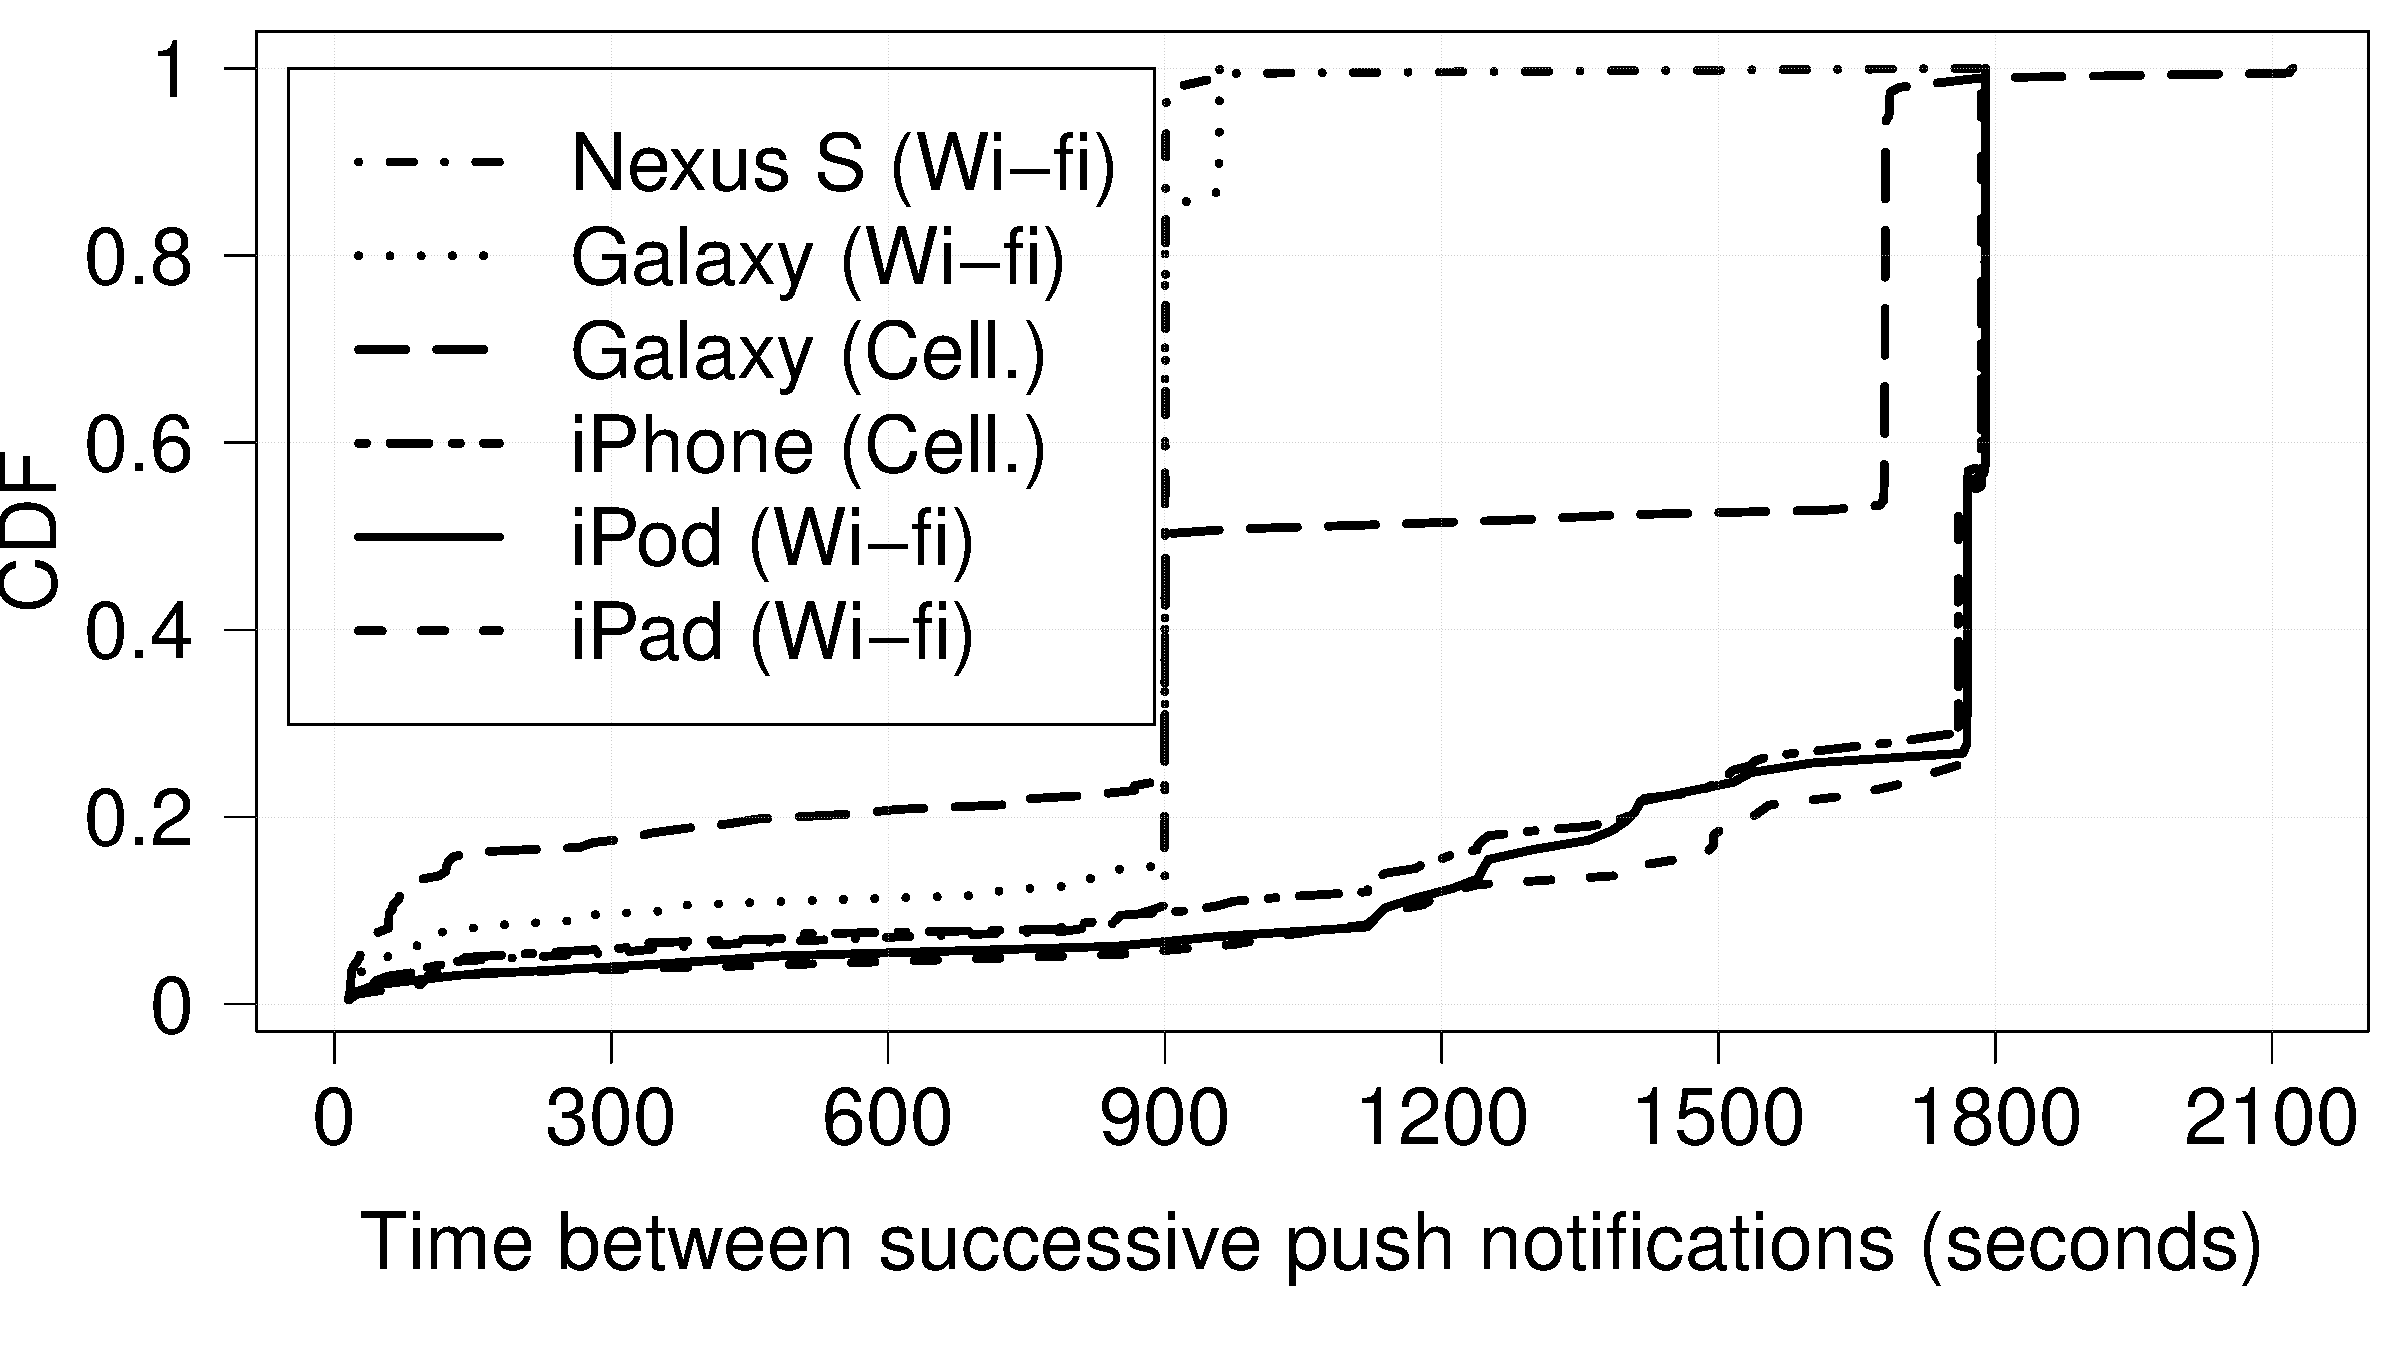
\includegraphics[width=\columnwidth]{plots/push_inter_arrival.pdf}
\caption{Inter-arrival time between push notification messages after factory reset. \emph{The iOS devices communicate with the notification server approximately once every 1800 seconds while the Android devices communicate once every 900 seconds with their notification server. \tbd{Add results from shen from iphone 3gs reset.}}}
\label{fig:inter-arrival-push}
\end{figure}

The push notifications messages, that contributed to the maximum traffic share in \fref{tab:traffic-share-factory-reset}, were exchanged over TCP. 
The iOS devices used TCP port 5223 while the Android devices used TCP port 5228 for the push notifications.
The notification services require a TCP connection to be established by the device and the server. 
The notification server uses this TCP connection to push notifications to the mobile device. 
The mobile device also periodically communicates with the notification server. 

In \fref{fig:inter-arrival-push} we plot the time between successive messages exchanged on the ports used for push notifications. 
We observe that the inter-arrival time between push notifications for the Android devices is 900 seconds for more than 80\% of the push notifications observed. 
For the iOS devices, we observe an inter-arrival time at least 1700~seconds for that more than 75\% of the push notifications. 
All Android flows with an inter-arrival time larger than 800 seconds consisted of an empty TCP packet sent by the device followed by a 25 byte payload sent by the server.
All iOS flows with an inter-arrival time larger than 1500 seconds began with an TCP packet with a payload of 85 bytes sent by the device followed by the server responding with of a TCP packet of 37 byte payload.

\subsection{Push Notifications In The Wild} 

We now characterize our observations on the push notifications we observed in the \moball dataset. 
The objective of this analysis was to answer the following questions
\begin{packedenumerate}
\item How frequently do Push notifications take place in the wild?
\item What is the impact of access technology on push notifications?
\item \tbd{What is the distribution of traffic volume of push notifications?}	
\item \tbd{How do push notifications change over OS and device upgrades?}
\item \tbd{Do not disturb -- How efficient are services like Do Not Disturb?}
\end{packedenumerate}

\begin{figure}
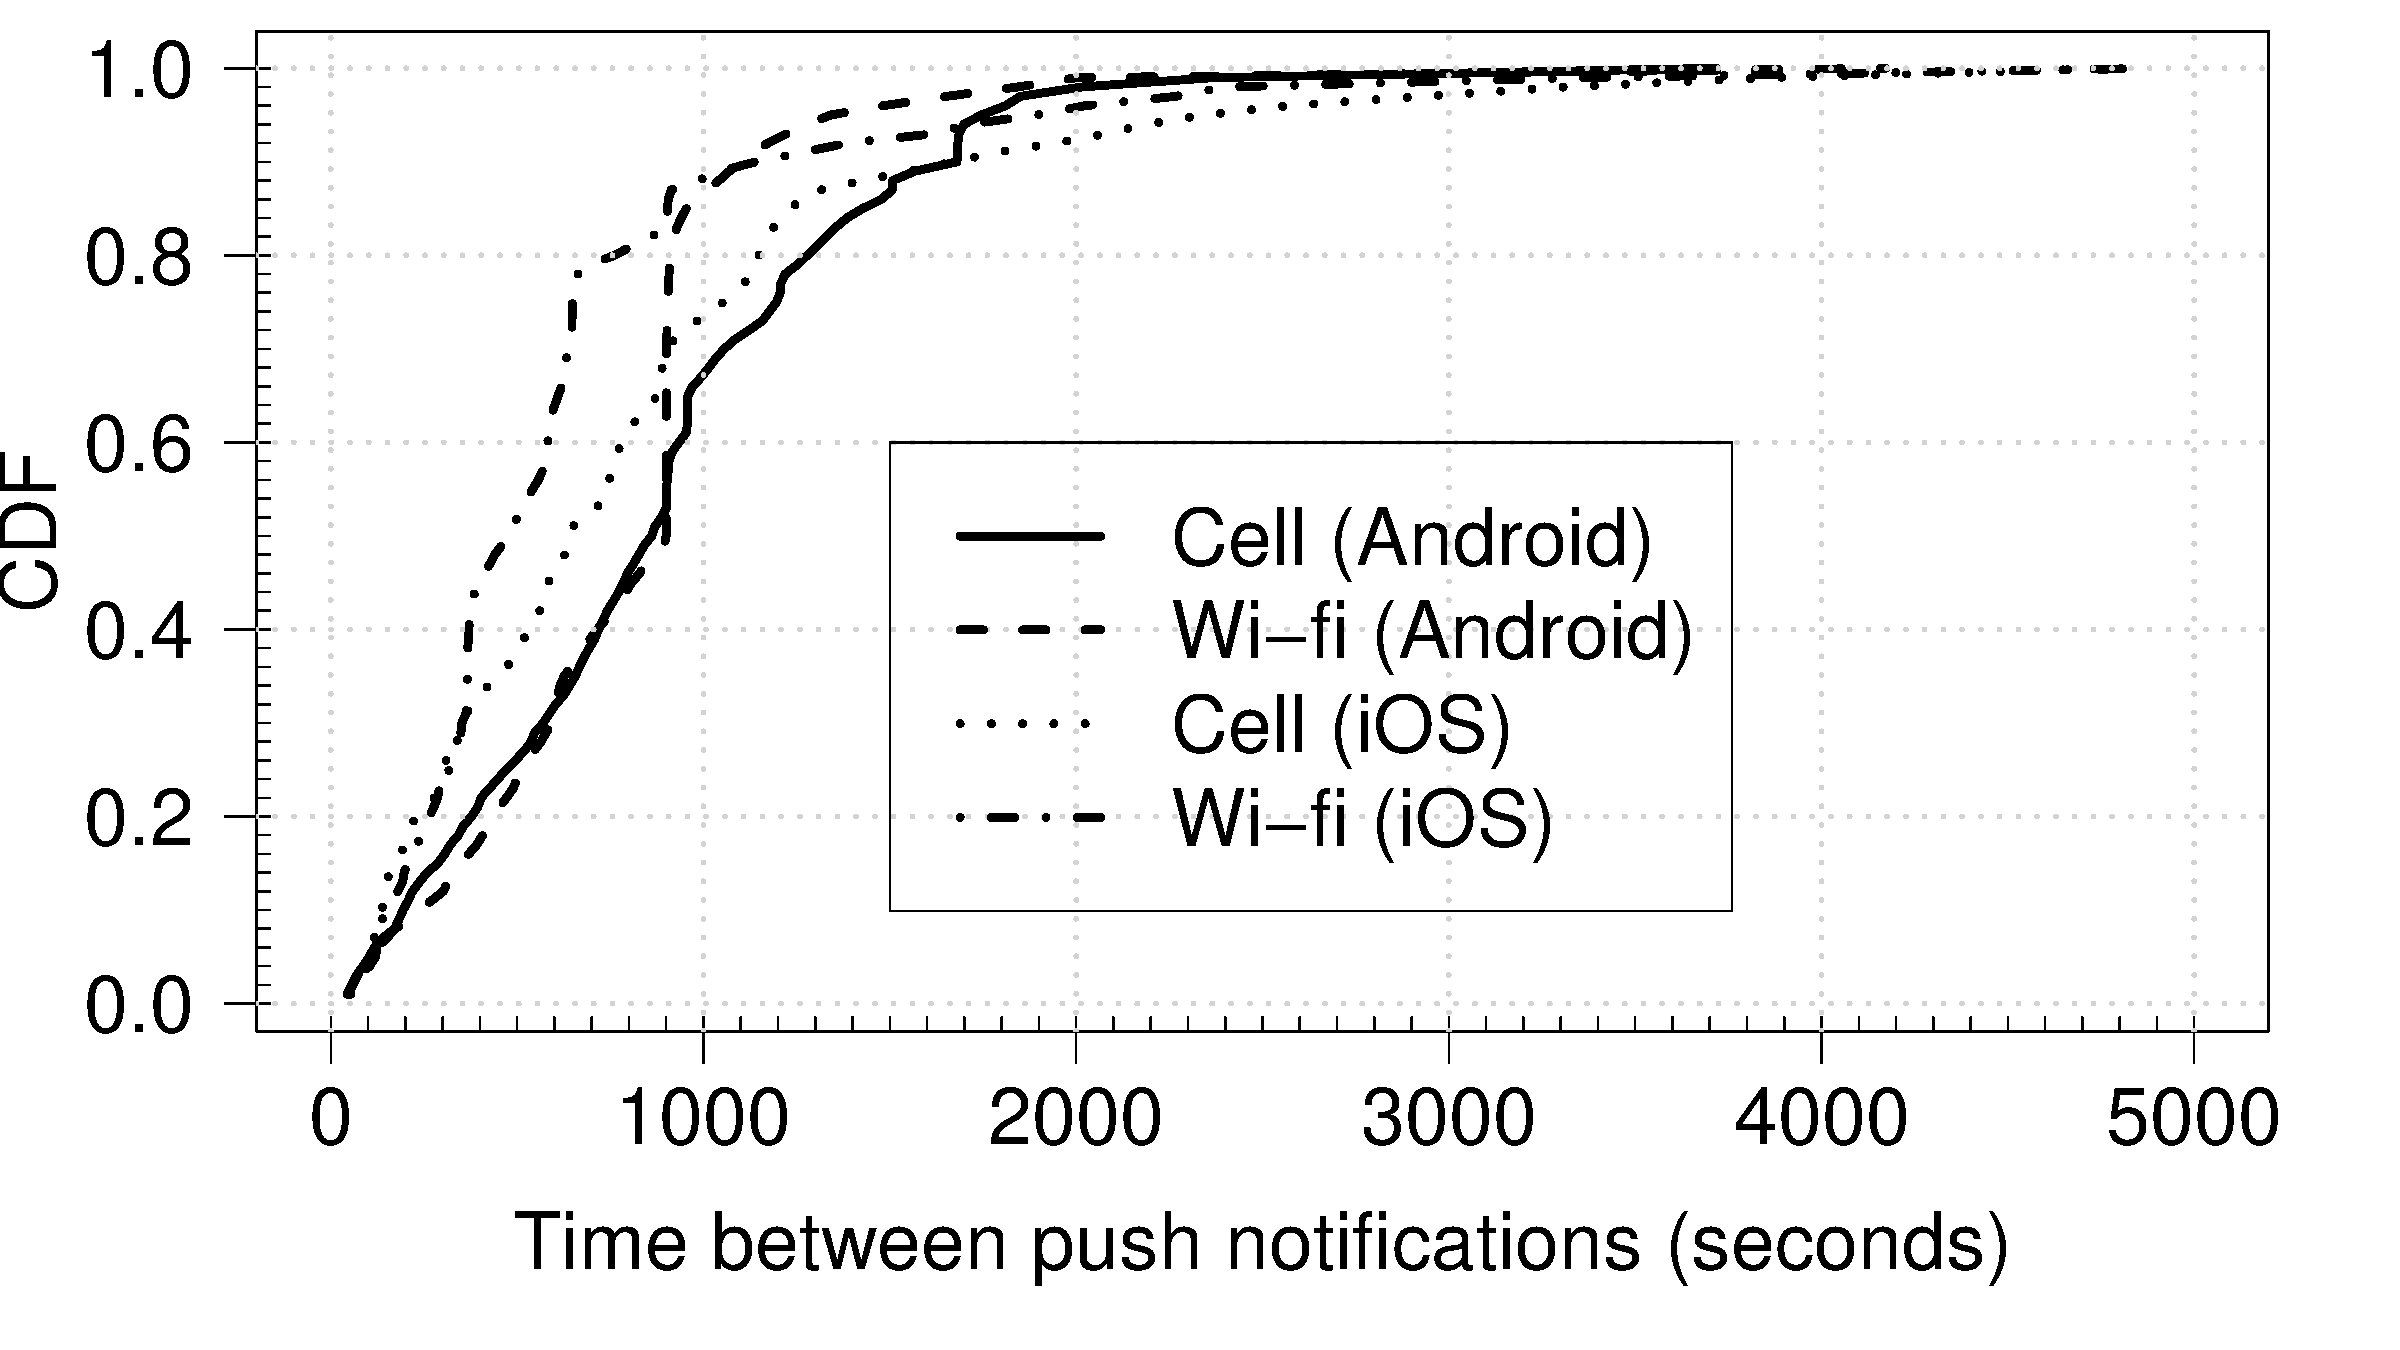
\includegraphics[width=\columnwidth]{plots/cdf_push_comparison_device_wild.pdf}
\caption{Distribution of the time between push notification messages in the wild. \emph{The frequency of push notification messages is higher for the iOS devices in our dataset compared to the Android devices. Notification messages are less frequent over cellular networks compared to Wi-Fi networks.}}
\label{fig:wild-cdf-push}
\end{figure}

%The advantage of \platname is that it allows for direct comparison between devices across and their behavior across access technologies. 
In \fref{fig:wild-cdf-push} we plot the distribution of the time between successive push notification messages for Android and iOS devices over cellular and \wifi networks. 
While computing this distribution, we account the diversity in device usage in the following manner.
For each device and each access technology we compute the 100 quantiles from 0.01 to 1.0 in steps of 0.01 of the time between successive push notifications. 
We then use the median value of each quantile (from 0.01 to 1.0 in steps of 0.01) for a given access technology and operating system of the device.
In \ref{fig:inter-arrival-push} we observe a higher time between push notifications on cellular networks compared to \wifi networks. 
We also observe that the time between push notifications is higher for the iOS devices in our dataset compared to the Android devices in our dataset. 
\tbd{The tcp ports used after the push notifications. Numbers for what fraction was ssl traffic at 443. and the servers to which the connection was made.}

\begin{figure}
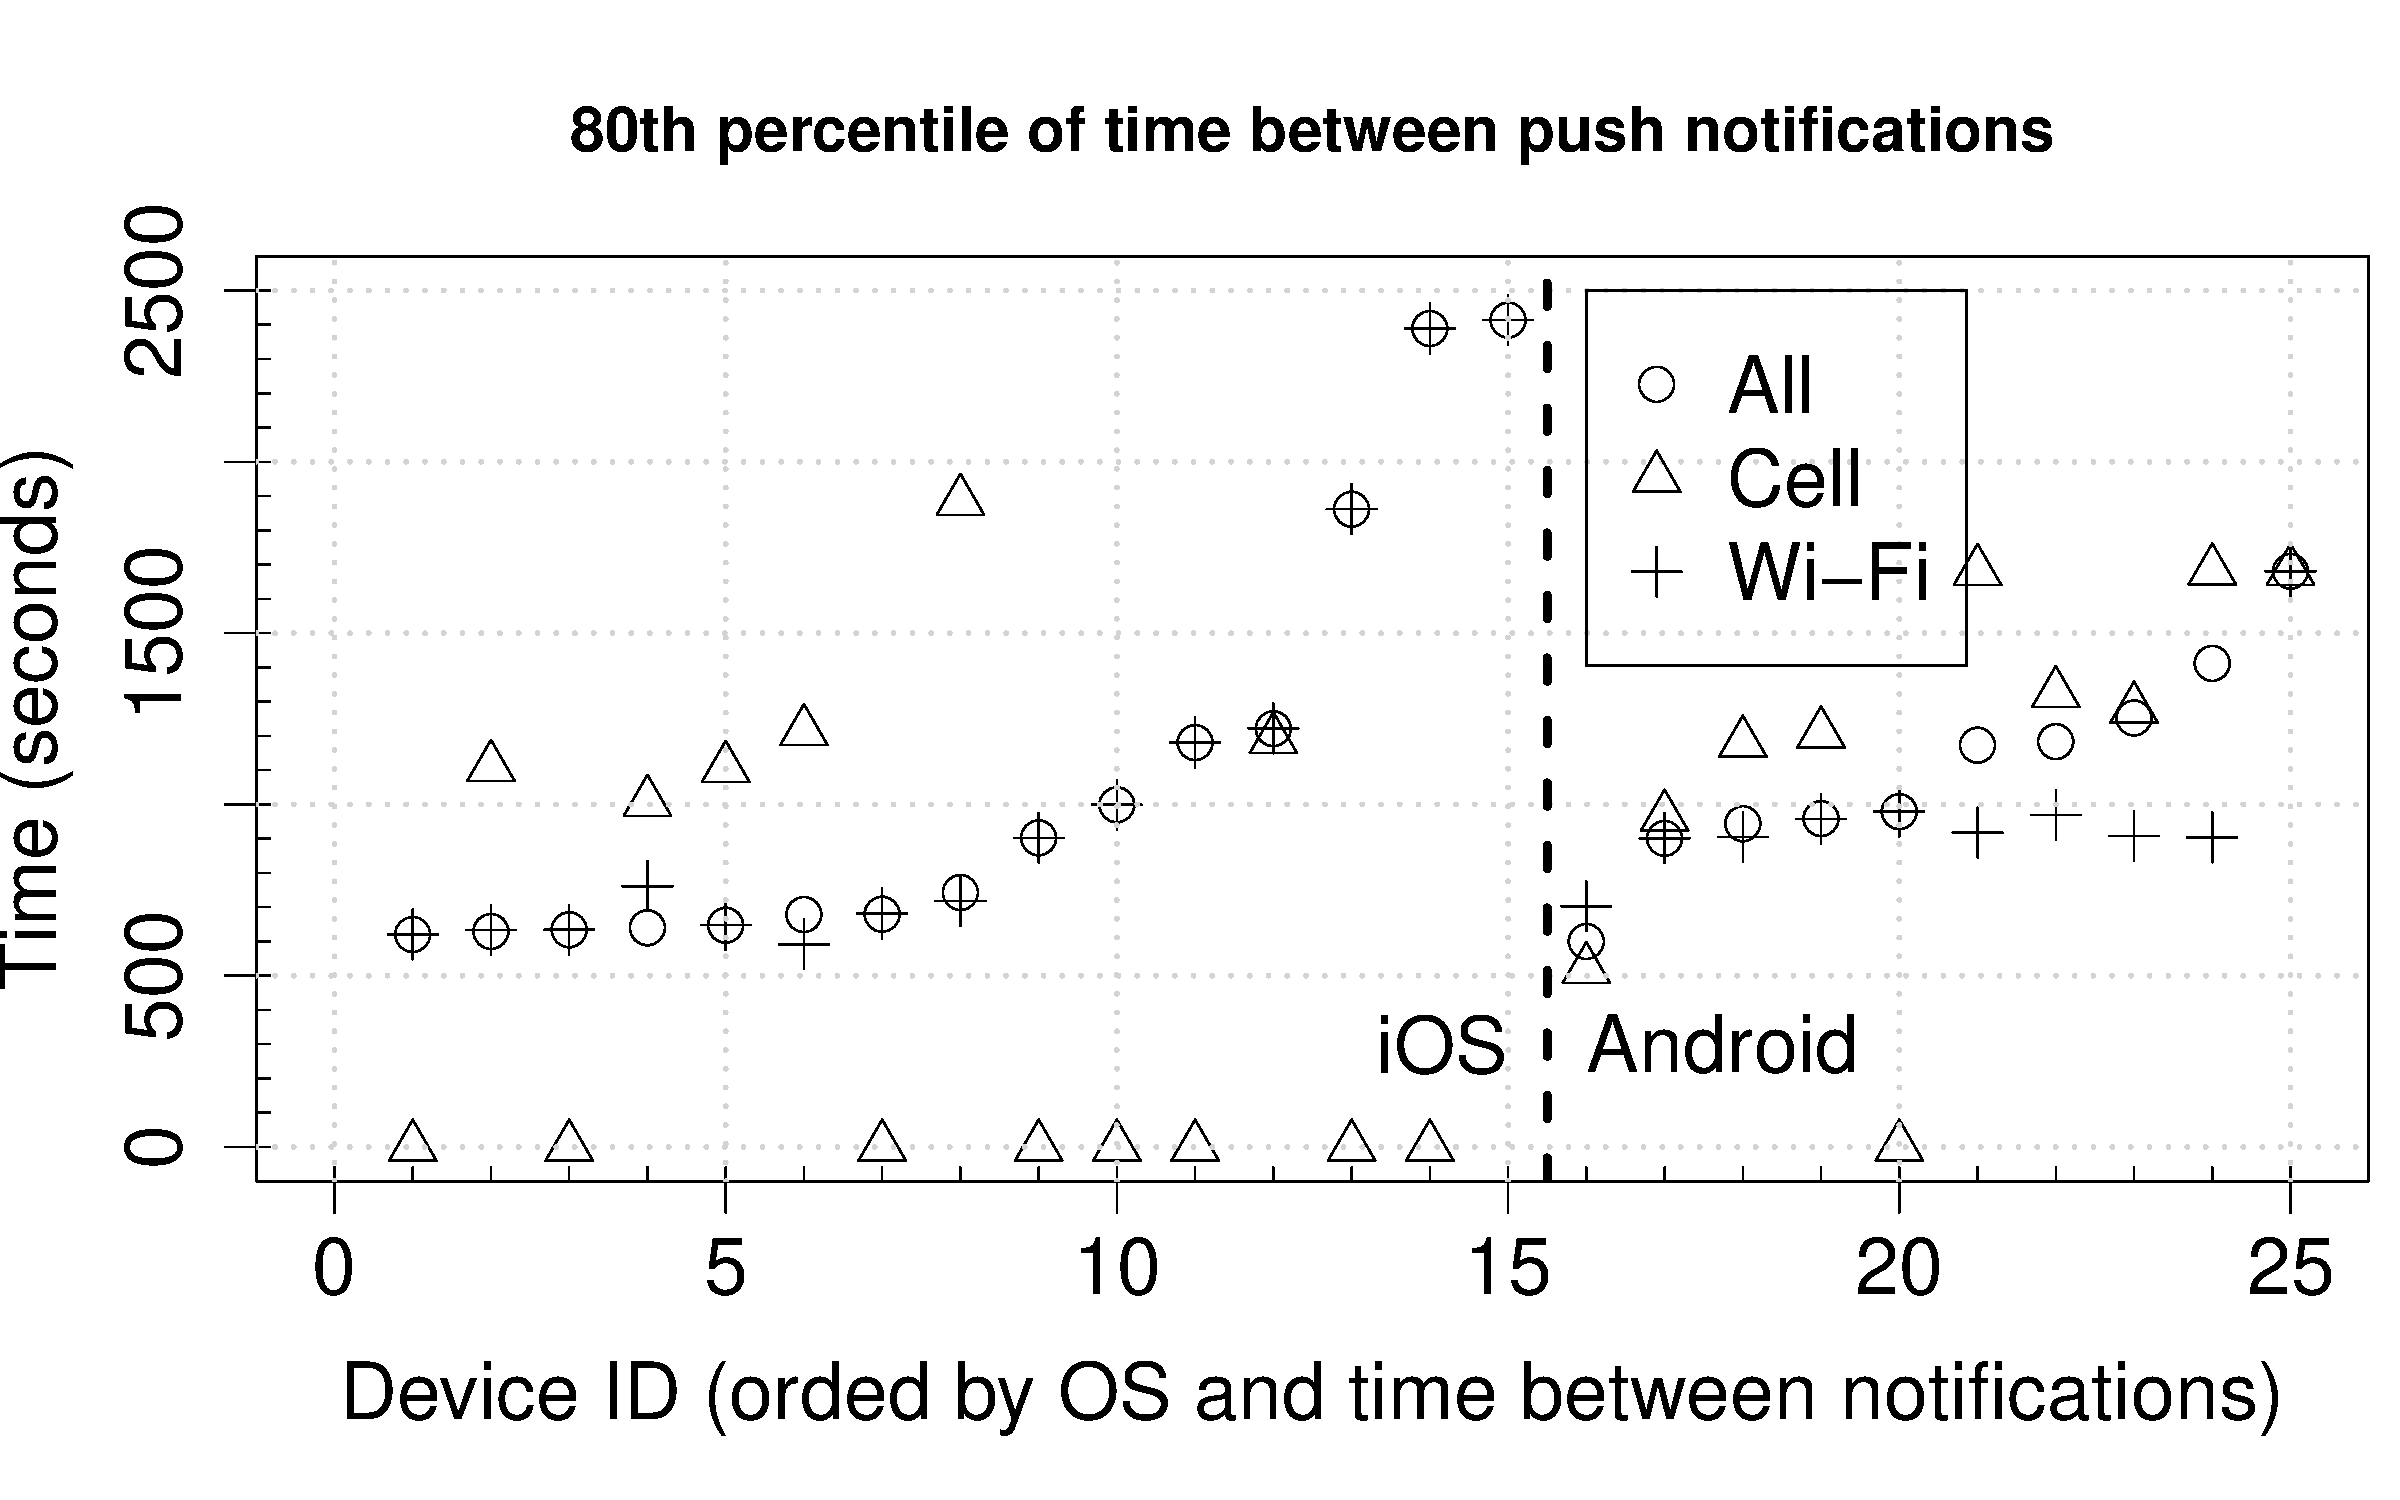
\includegraphics[width=\columnwidth]{plots/push_inter_arrival_wild.pdf}
\caption{Inter-arrival time between push notifications in the wild. \emph{Push notifications occur less frequently over Cellular networks. The rate of push notifications depends on users and the applications installed. \tbd{DISCUSS: Better representation for tablets -- currently they have a value of 0 for the cell networks.}}}
\label{fig:wild-inter-arrival-push}
\end{figure}


In \fref{fig:wild-inter-arrival-push} we present the time between successive push notifications for the 25 devices in our dataset. 
As observed in \fref{fig:wild-cdf-push} we observe that the iOS devices receive push messages more frequently that the Android devices. 
We also observe that the time between push notifications is higher for Android devices.
The iOS devices prefer a cellular data connection for Push notification over \wifi \tbd{http://support.apple.com/kb/TS4264}. 
However, in \fref{fig:wild-cdf-push} and \fref{fig:wild-cdf-push} despite this preference, we observe that the time between successive push notifications for iOS devices is higher over cellular networks in comparison to \wifi networks.  
We observe that \tbd{SSL traffic} to mail servers was followed \tbd{x\%} after push notifications.
This implies that higher usage of the device over \wifi may result in a higher number of notificatons received. 
In \fref{fig:wild-inter-arrival-push}, device ID 
%Only if the cellular connection is not available or viable will the device switch to Wi-Fi for APNs connections.


\begin{figure}
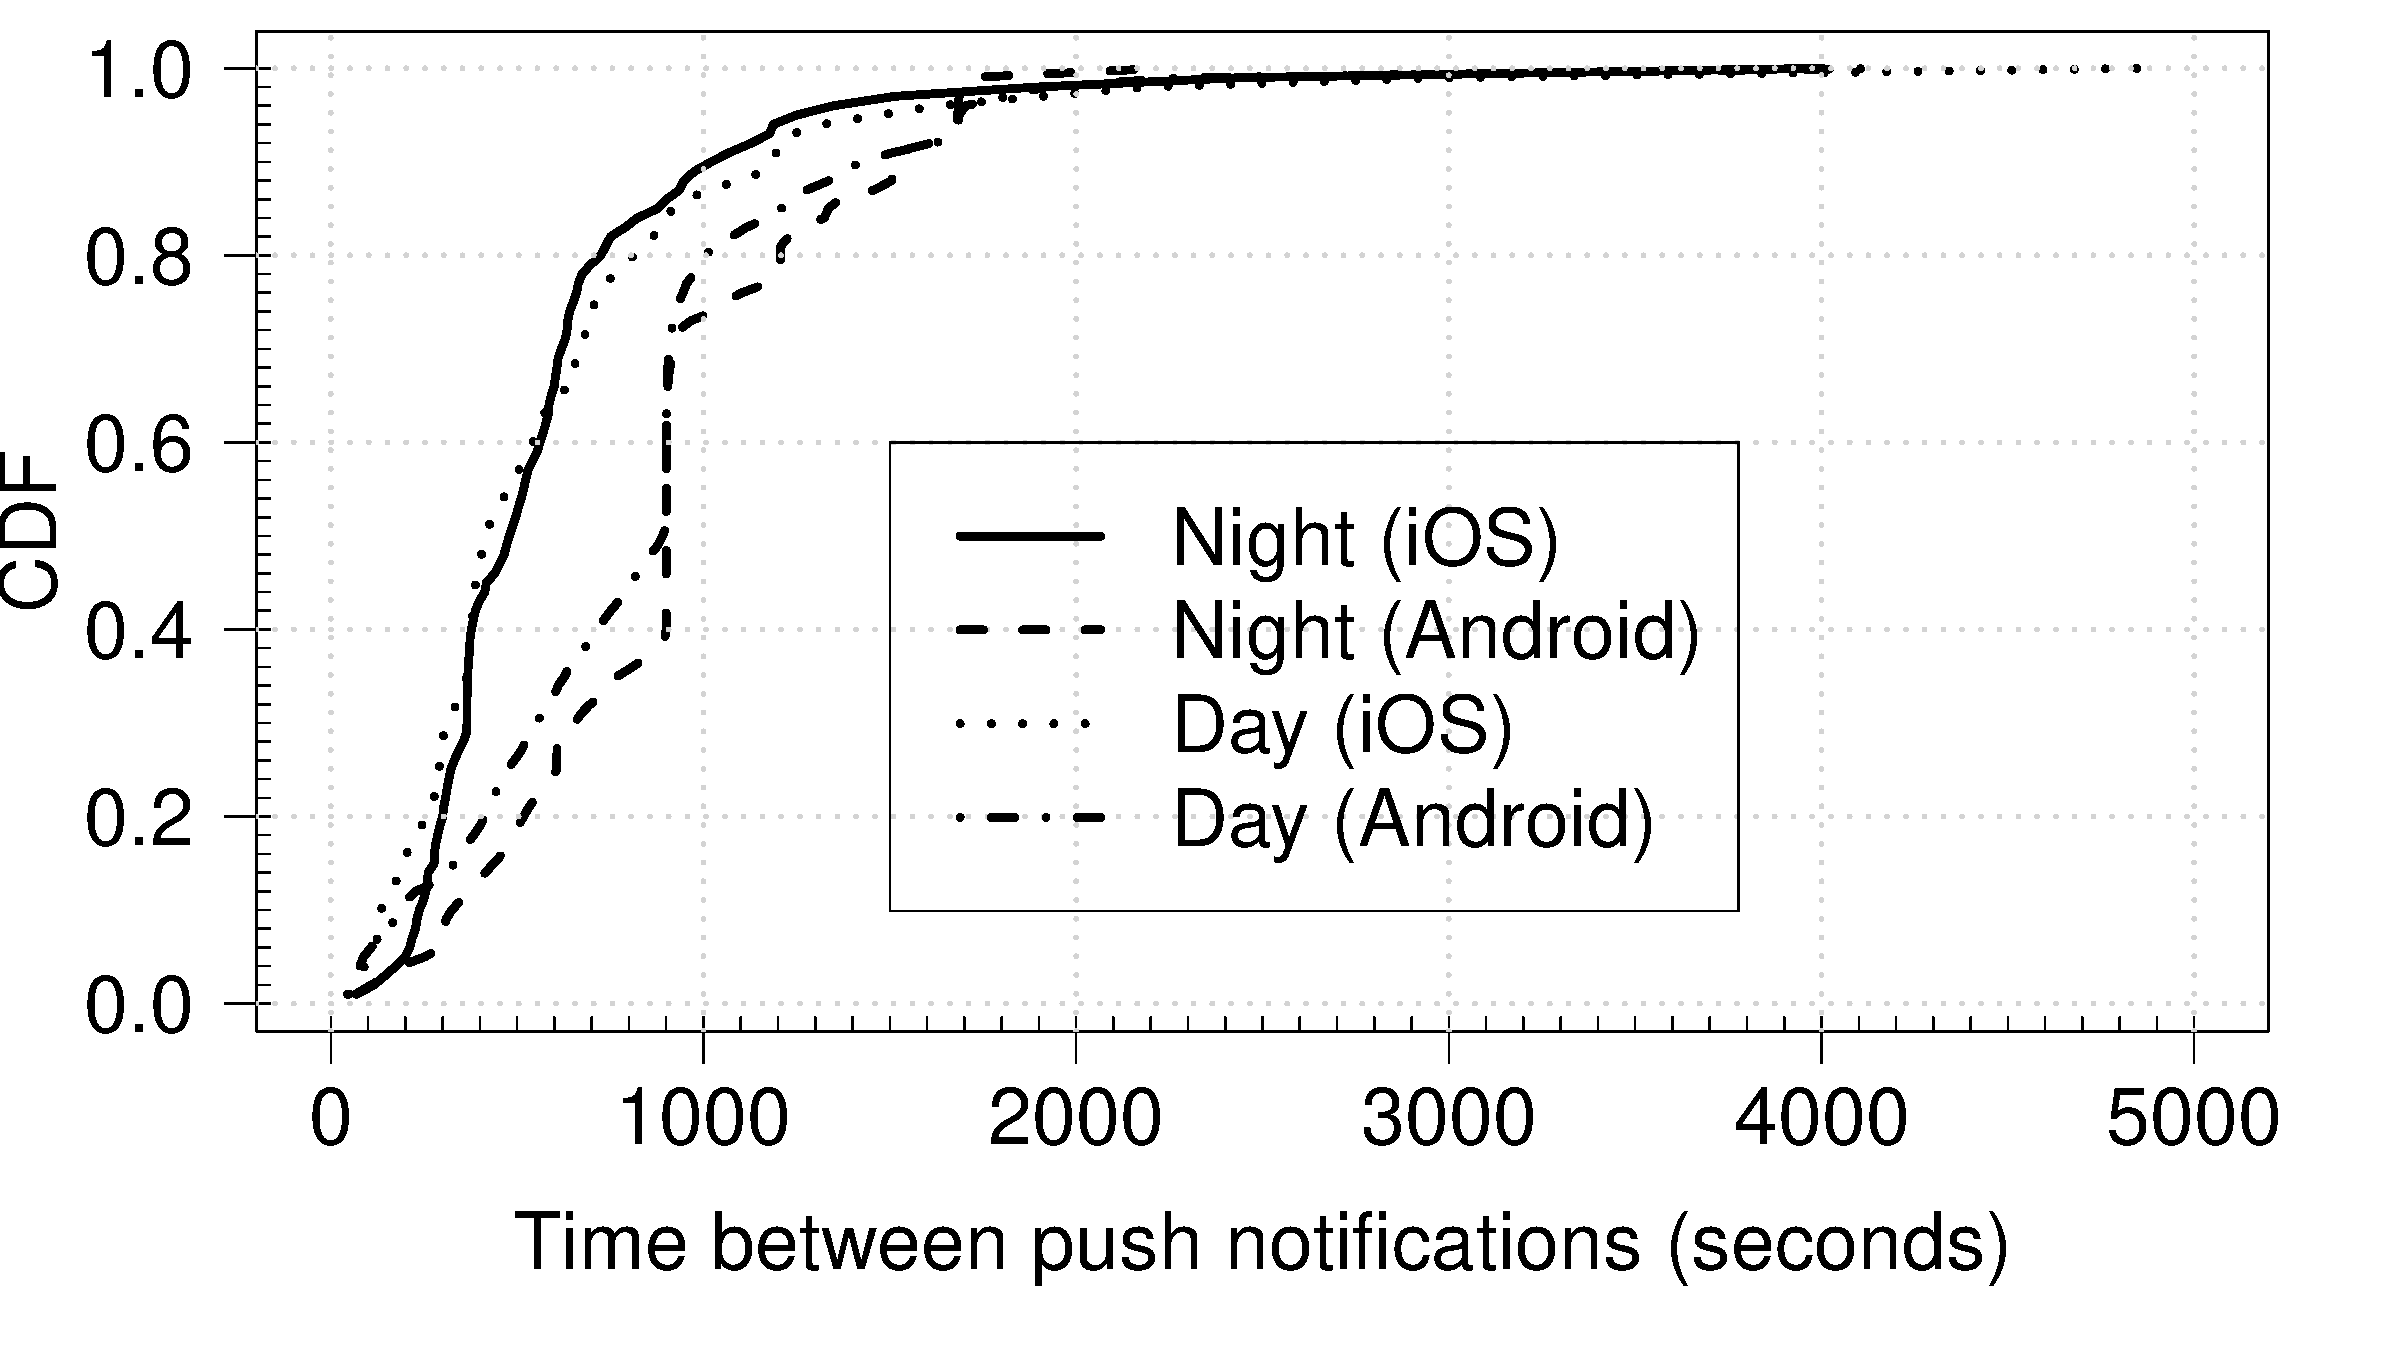
\includegraphics[width=\columnwidth]{plots/cdf_night_push_comparison_device_wild.pdf}
\caption{Impact of time-of-day on the push notifications. \emph{The rate of push notifications is agnostic of the time of the day for iOS devices.}}
\label{fig:wild-cdf-push-night}
\end{figure}

\tbd{Highlight the pervasive nature of \platname  allows us}
We now use \fref{fig:wild-cdf-push-night} we to show that the push notification are agnostic of the time of the day. 
For \fref{fig:wild-cdf-push-night}, we consider two time periods: from midnight to 6 am (\emph{Night}) and from 6 am to midnight (\emph{Day}).
The values used in the distributions is computed using the technique used for \ref{fig:wild-cdf-push}. 
We observe that the Android and iOS devices exhibit a similar behavior that appears to be agnostic of the time of the day. 
The iOS devices (from verion 6.0) come with a feature called \emph{Do Not Disturb (DND)} that does raise notification alarms on receiving notifications during specific time periods. 
We also observe that during the intervals configured as \emph{Do Not Disturb}, notification messages were exchanged by devices that used this feature enabled. 

\tbd{Who is pushing the notifications. Servers used for push notifications..based on DNS requests responses}

\subsection{Location Services In The Wild}


\subsection{Discussion}



